\chapter{Background e Stato dell'Arte}
In questo capitolo vengono introdotti i concetti fondamentali necessari per comprendere il contesto in cui si inserisce il lavoro di tesi. Il contenuto di questa sezione si articola su tre punti cardine: l'evoluzione e l'architettura dei Large Language Models, introducendo e illustrando la struttura dei Transformer e dello spazio latente; il ruolo di tali modelli nell'ambito della sicurezza del software per la Vulnerability Detection ed infine, la tassonomia degli attacchi avversari adottati nello studio ed una presentazione alle basi della Mechanistic Interpretability per l'analisi delle rappresentazioni interne.

\section{Fondamenti su LLM}
Un Large Language Model (LLM) è una rete neurale di grandi dimensioni addestrata su enormi quantità di testo per comprendere e generare linguaggio naturale. Gli LLM sono progettati per generare, riassumere, tradurre e analizzare testo in diversi contesti. Questo li rende la base tecnologica dietro ai moderni chatbot e assistenti virtuali \cite{Definizione_LLM}.

\subsection{Cos'è un LLM e il concetto di Large}
Tipicamente, con il termine \textit{large Language Models} (LLMs) ci si riferisce a modelli di linguaggio basati su architetture Transformer che contengono miliardi di parametri o più, i quali sono addestrati su quantità di testo massivo, come per GPT-3, PaLM, Galactica e LLaMA. Gli LLM hanno dimostrato avere forti capacità nel comprendere il linguaggio naturale e risolvere compiti complessi tramite generazione testuale.

Attualmente gli LLM sono principalmente costruiti sulla base dell'architettura Transformer, dove i layer di attenzione sono impilati in una rete neurale molto profonda.
Il concetto di Large negli LLM non presenta una definizione accademica rigorosa, ma si riferisce fondamentalmente ad un drastico salto di ordine di grandezza (scaling) sotto tre dimensioni principali:

\begin{itemize}
    \item \textbf{Numero di parametri:} i parametri sono i pesi (weights) e i bias della rete neurale, ovvero i valori numerici che il modello aggiorna durante la fase di apprendimento. Il termine Large entra in gioco con il passaggio da milioni di parametri a miliardi. I primi modelli pre-addestrati presentavano tra i 110 e i 340 milioni di parametri, mentre modelli come GPT-3 ne contano circa 175 miliardi.
    \item \textbf{Le dimensioni del dataset:} per evitare casi di overfitting addestrando modelli con miliardi di parametri, è necessario addestrarli su dataset di dimensioni enormi, che contengono centinaia di miliardi di token. Questi dataset sono spesso raccolti da fonti web, libri, articoli e altri tipi di testo. La dimensione del dataset è un fattore chiave per garantire che il modello possa generalizzare bene e non semplicemente memorizzare i dati di addestramento.
    \item \textbf{Le risorse computazionali:} anche le risorse computazionali necessarie per addestrare i modelli composti da molteplici GPU che lavorano in parallelo per un tempo esteso contribuiscono alla definizione di Large. L'addestramento di modelli con miliardi di parametri richiede infrastrutture di calcolo avanzate, come cluster di GPU o TPU, e può richiedere settimane o mesi per completare l'addestramento.
\end{itemize}

\subsection{L'evoluzione negli anni}
Negli ultimi anni, gli LLM hanno subito un'evoluzione significativa, passando da modelli relativamente piccoli a modelli con miliardi di parametri. Questa crescita ha portato a miglioramenti nelle capacità di comprensione e generazione del linguaggio, ma ha anche introdotto nuove sfide in termini di sicurezza e vulnerabilità.
Tecnicamente, la modellazione del linguaggio (LM) rappresenta uno dei principali approcci per far progredire l'intelligenza linguistica delle macchine. In generale, un modello di linguaggio mira a modellare la probabilità generativa di sequenze di parole, così da predire le probabilità dei token futuri.
La ricerca sui modelli di linguaggio ha ricevuto molte attenzioni nella letteratura, tanto da poter essere divisa in quattro periodi principali di sviluppo \cite{surveylargelanguagemodels} :
\begin{itemize}
    \item \textbf{Statistical language models (SLM):} sono stati sviluppati negli anni '90 basandosi su metodi di apprendimento statistico. L'idea era quella di modellare la predizione delle parole basandosi sulle assunzioni di Markov, predicendo la prossima parola sfruttando il contesto più recente. Questi modelli, sono stati ampiamente utilizzati per migliorare le prestazioni in Information Retrieval (IR) e in Natural Language Processing (NLP).
    Tuttavia questi modelli soffrono spesso di problemi legati alla dimensionalità: è difficile stimare accuratamente modelli di linguaggio di ordine elevato, poiché è necessario stimare un numero esponenziale di probabilità di transizione.
    \item \textbf{Neural language models (NLM):} i modelli di linguaggio neurali (NLM) modellano la probabilità delle sequenze di parole attraverso l'uso di reti neurali, come ad esempio il perceptron multistrato (MLP) e le reti neurali ricorrenti (RNN). Un notevole contributo è quello di aver introdotto il concetto di rappresentazione distribuita (distributed representation) delle parole e aver costruito la funzione di predizione della parola condizionata dalle caratteristiche aggregate del contesto.
    In seguito, word2vec ha introdotto un nuovo approccio per la costruzione di una rete neurale shallow, ovvero a un solo hidden layer, per imparare le rappresentazioni distribuite delle parole, migliorando così l'efficienza tra una varietà di attività NLP. Questi studi hanno iniziato l'uso dei language models per il representation learning, avendo quindi un importante impatto nel campo dell'NLP.
    \item \textbf{Pre-trained language model (PLM):} Come primo tentativo, ELMo è stato proposto per catturare rappresentazioni delle parole dinamiche e sensibili al contesto (context-aware), effettuando prima il pre-addestramento (pre-training) di una rete LSTM bidirezionale (biLSTM) invece di apprendere rappresentazioni fisse delle parole e successivamente il fine-tuning della rete biLSTM su specifici task a valle (downstream task). Inoltre, basandosi sull'architettura Transformer, che è altamente parallelizzabile e dotata di meccanismi di self-attention, è stato proposto BERT, il quale pre-addestra modelli di linguaggio bidirezionali tramite task di pre-addestramento appositamente progettati su corpora di grandi dimensioni e non etichettati. Queste rappresentazioni contestuali e pre-addestrate delle parole si rivelano molto efficaci come feature semantiche di uso generale, innalzando notevolmente gli standard prestazionali nei task di NLP. Questo studio ha ispirato un gran numero di lavori successivi, stabilendo il paradigma di apprendimento basato su "pre-training e fine-tuning". Seguendo questo paradigma, è stato sviluppato un elevato numero di studi sui modelli di linguaggio pre-addestrati (PLM), che hanno introdotto architetture differenti (es. GPT-2 e BART) oppure strategie di pre-addestramento migliorate. In tale paradigma, è spesso necessario effettuare il fine-tuning del PLM per adattarlo ai diversi downstream task.
    \item \textbf{Large Language Models (LLM):} I ricercatori osservarono che lo scaling dei Pre-trained Language Models (PLM) porta spesso a una migliore capacità del modello nei downstream task.
    Sebbene lo scaling venga applicato principalmente alle dimensioni del modello, mantenendo architetture e task di pre-addestramento simili, questi PLM di grandi dimensioni mostrano comportamenti differenti rispetto ai PLM più piccoli (ad es., BERT da 330 milioni di parametri e GPT-2 da 1,5 miliardi di parametri) e rivelano abilità sorprendenti nella risoluzione di una serie di task complessi. Ad esempio, GPT-3 è in grado di risolvere task few-shot attraverso l'apprendimento nel contesto (in-context learning), mentre GPT-2 non ottiene buoni risultati. Di conseguenza, la comunità scientifica ha coniato il termine 'modelli di linguaggio di grandi dimensioni (LLM)' per questi PLM su larga scala, i quali stanno attirando una crescente attenzione da parte della ricerca.
\end{itemize}

Il concetto di modello di linguaggio non è una novità tecnica specifica degli LLM, ma si è evoluto nel corso dei decenni di pari passo con i progressi dell'intelligenza artificiale. I primi modelli di linguaggio miravano principalmente a modellare e generare dati testuali, mentre i modelli di linguaggio più recenti, ad esempio GPT-4, si concentrano sulla risoluzione di task complessi. Questo passaggio, dalla modellazione del linguaggio alla risoluzione di task, rappresenta un importante salto nel pensiero scientifico, che costituisce la chiave per comprendere lo sviluppo dei modelli di linguaggio nella storia della ricerca.
Il concetto stesso di "Large" si è evoluto attraverso l'architettura Mixtrue of Experts (MoE): durante la generazione di un singolo token, un meccanismo di routing attiva solo una piccola frazione dei parametri totali del modello, consentendo così di scalare a modelli con trilioni di parametri senza aumentare proporzionalmente i costi computazionali. 

\subsection{L'architettura di un Transformer e il Meccanismo di Attenzione} 
L'architettura Transformer è stata introdotta da Vaswani et al. nel 2017 nel paper \textit{Attention is All You Need} \cite{attention_is_all_you_need} ed è stata la chiave di volta per lo sviluppo dei modelli di linguaggio di grandi dimensioni.
Nel paper originale viene presentata un'architettura composta da un encoder e un decoder \ref{fig:Transformer}: l'encoder mappa una sequenza di simboli in input $(x_1, ..., x_n)$ in una rappresentazione continua $z = (z_1, ..., z_n)$. Dato $z$ il decoder genera un output  $y_1,..., y_m$ come una sequenza di simboli, un elemento alla volta. Il decoder è auto-regressivo, ovvero predice il token successivo basandosi sui token precedenti, consumando i simboli generati precedentemente come input addizionale per quello successivo.

\begin{figure}[H]
    \centering
    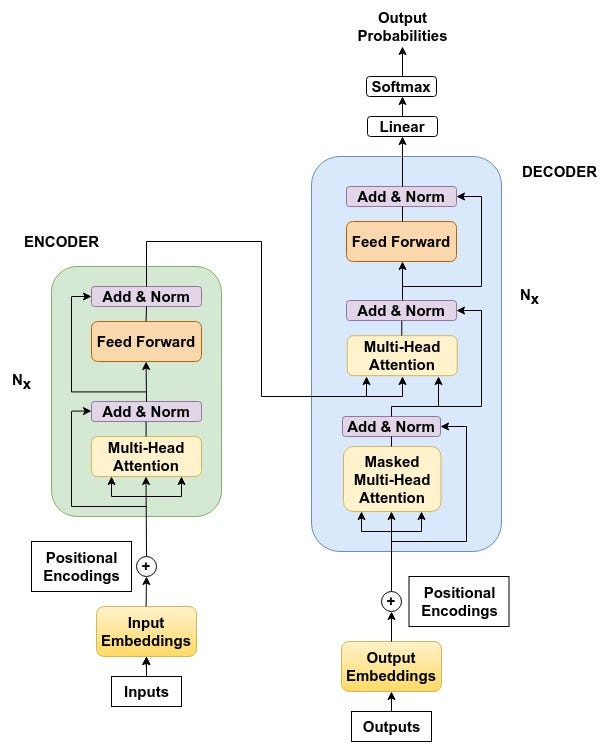
\includegraphics[width=0.45\textwidth]{immagini/encoder_decoder.jpg}
    \caption{L'architettura di un Transformer Encoder-Decoder.}
    \label{fig:Transformer}
\end{figure}

Sebbene il Transformer originale fosse basato su un'architettura bidirezionale di tipo Encoder-Decoder, i modelli linguistici moderni utilizzano un approccio di tipo Decoder-only, eliminando completamente l'Encoder e utilizzando solo il Decoder.
Non esiste quindi più una separazione netta tra "fase di lettura" e "fase di scrittura": il modello considera l'input iniziale, il prompt, e la risposta del modello stesso come un'unica grande sequenza di testo continuo.

Il Decoder è composto da più strati sequenziali, chiamati layer. 
Rispetto all'architettura originale del 2017,oggi ogni layer del Transformer è composto da soli due sottostrati (sub-layer): la Self-Attention e una rete Feed-Forward (FFN) che utilizza funzioni di attivazione come SwiGLU o GeLU; versioni più efficienti rispetto alla vecchia ReLU proposta nel paper originale.
Anche il flusso interno dei dati ha subìto un'ottimizzazione: oggi si preferisce normalizzare l'input prima che entri nei sub-layer (approccio Pre-LN), utilizzando varianti più snelle e veloci da calcolare come la RMSNorm (Root Mean Square Normalization), che sostituisce la standard Layer Normalization.
C'è però un aspetto cruciale che è rimasto intatto dal 2017 a oggi: il mascheramento causale (causal masking). Questo meccanismo impedisce rigorosamente all'algoritmo di "guardare nel futuro", garantendo che il modello, sia in fase di addestramento che di generazione vera e propria, impari a predire il token successivo basandosi esclusivamente su quelli che lo precedono.

\begin{figure}[H]
    \centering
    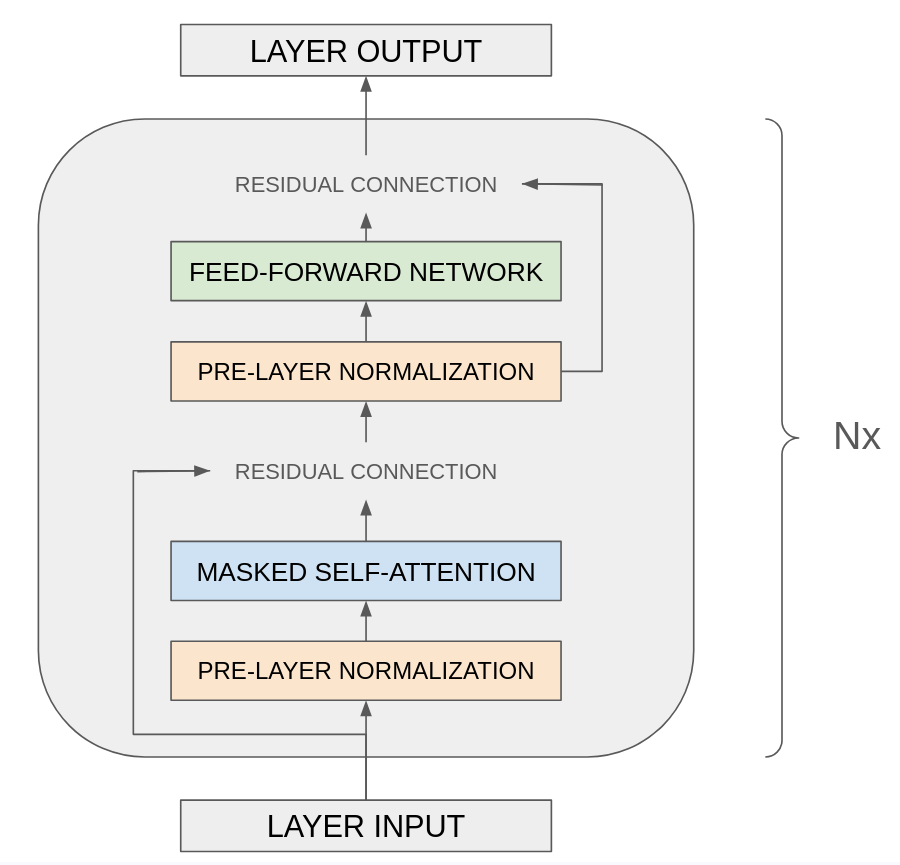
\includegraphics[width=0.45\textwidth]{immagini/decoder_only.png}
    \caption{L'architettura di un Transformer Decoder-only.}
    \label{fig:Transformer-DecoderOnly}
\end{figure}

Al fine di comprendere il funzionamento di un LLM, è fondamentale esporre l'architettura dei layer del decoder.
Per migliorare la stabilità di training viene utilizzato un layer di \textbf{pre-normalizzazione}: l'input viene normalizzato per ogni sub-layer del transformer invece di normalizzare l'output. Possono essere utilizzate diverse tecniche di normalizzazione come la RMSNorm.
Le funzioni di attivazioni tipicamente adottate sono la SwiGLU (Swish-Gated Linear Unit) o la GeLU: in particolar modo la SwiGLU ha una curva matematica che non azzera in modo netto i valori negativi, ma li attenua gradualmente e attraverso l'uso di gate decide quali informazioni lasciare passare. \cite{LLama_layer}

Il meccanismo di attenzione è il cuore dell'architettura Transformer. Esso consente al modello di pesare dinamicamente l'importanza di diverse parti dell'input quando genera una risposta. Nello specifico, la self-attention permette al modello di considerare tutte le parole in una frase o in un contesto più ampio, assegnando loro pesi diversi a seconda della loro rilevanza per il compito specifico. In particolar modo la funzione di attenzione può essere descritta come una mappatura di una query e un set di coppie chiave-valore ad un output, dove la query, le chiavi, valori e output sono tutti vettori. L'output è quindi calcolato come una somma pesata dei valori, dove il peso assegnato ad ogni valore è calcolato applicando una funzione di compatibilità della query con la chiave corrispondente.

Nel dettaglio ci si riferisce all'attenzione con il nome di \textbf{Scaled Dot-Product Attention}, dove l'input è formato dalle query e dalle chiavi di dimensione $d_k$, e dai valori di dimensione $d_v$, dove con $d$ ci si riferisce alla dimensione dei vettori. Viene calcolato il prodotto scalare tra le query con tutte le chiave, ciascuno diviso per $\sqrt{d_k}$, e applicando una funzione softmax per ottenere i pesi sui valori.

Un altro aspetto fondamentale dei transformer è l'attenzione multi-testa (multi-head attention), che consente al modello di prestare attenzione congiuntamente a diversi sottospazi di rappresentazione in diverse posizioni. In questo modo, il modello può catturare diversi tipi di relazioni tra le parole e i concetti.
Questo meccanismo può essere suddiviso in tre fasi:
\begin{enumerate}
\item \textbf{Proiezione e sdoppiamento:} le matrici di Query, Key e Value vengono proiettate linearmente per $h$ volte, dove $h$ è il numero di teste di attenzione, creando così $h$ versioni diverse e compatte delle query, chiavi e valori. Ognuna di queste versioni rappresenta una "testa" (head) di attenzione.
\item \textbf{Calcolo in parallelo:} viene calcolata in parallelo la Scaled Dot-Product su ciascuna delle $h$ teste.
\item \textbf{Concatenazione e output}: gli $h$ risultati ottenuti vengono concatenati tra loro e moltiplicati per un'ultima matrice di pesi, generando i valori dell'output finale.  
\end{enumerate}

La multi-head attention nel decoder permette ad ogni posizione nel decoder di prestare attenzione a tutte le posizioni precedenti fino a quella posizione. Bisogna prevenire l'information flow da posizioni future, per preservare la proprietà auto-regressiva del modello. Per questo motivo, viene applicato un mascheramento causale (causal masking) durante lo scaled dot-product attention impostando a $-\infty$ i valori delle connessioni illegali prima di applicare la funzione softmax.

\subsection{Rappresentazioni Vettoriali e Spazio Latente}
Gli LLM rappresentano il testo in uno spazio vettoriale ad alta dimensione, noto come spazio latente. In questo spazio, le parole, le frasi e i concetti sono rappresentati come vettori numerici, che catturano le relazioni semantiche tra di essi. Ad esempio, parole con significati simili tendono ad essere rappresentate da vettori vicini nello spazio latente, mentre parole con significati diversi sono rappresentate da vettori più distanti. Questa rappresentazione consente al modello di comprendere e generare testo in modo più efficace, poiché può sfruttare le relazioni semantiche tra le parole per produrre risposte coerenti e pertinenti.

Il primo passo per poter introdurre il concetto di rappresentazioni vettoriali è quello di definire il concetto di token: l'unità fondamentale di testo che un modello di linguaggio elabora.
Questo è una sequenza di caratteri che può rappresentare una parola, una parte di parola o anche un carattere singolo a seconda del contesto.

Per poter generare un token vengono utilizzati algoritmi come \textbf{Byte Pair Encoding (BPE)}, una tecnica di compressione dati che iterativamente rimpiazza le coppie di byte più frequenti in una sequenza con un singolo byte inutilizzato. Nel contesto dei modelli di linguaggio, BPE viene utilizzato per suddividere il testo in token, dove, invece di unire le coppie di bytes più frequenti, vengono uniti caratteri o sequenze di caratteri.
Viene inizializzato il simbolo del vocabolario con i caratteri individuali, viene poi rappresentata ogni parola come una sequenza di caratteri ed un simbolo speciale di fine parola, il quale permette di ripristinare la parola originale. Successivamente vengono contate le coppie di simboli e ogni occorrenza della coppia più frequente viene sostituita con un nuovo simbolo.
Ogni operazione di merge produce un nuovo simbolo che rappresenta un $n$-gramma di caratteri.
Il nuovo token viene quindi aggiunto al vocabolario ed il processo di conteggio e fusione viene ripetuto iterativamente, espandendo il vocabolario con nuovi token sempre più lunghi.
L'algoritmo termina quando viene raggiunta la dimensione del vocabolario prefissata.\cite{sennrich2016neuralmachinetranslationrare}
Per ovviare ai limiti del BPE, la ricerca si sta spostando verso architetture Token-Free o Byte-Level, rendendo i modelli nativamente multilingue.

Strettamente collegato al concetto di token c'è quello di embedding: ovvero vettori di numeri reali che codificano il significato di un oggetto in un formato che può essere elaborato da un modello di machine learning. Formalmente è il risultato di una funzione $f: X \rightarrow \mathbb{R}^n$ che mappa uno spazio discreto $X$, come parole, documenti o immagini, in uno spazio vettoriale continuo di dimensione $n$, preservando relazioni semantiche come distanza e direzione. \cite{cosa_sono_gli_embeddings} 
Il flusso per generare gli embedding inizia con la tokenizzazione del testo fornito al modello, che suddivide il testo in token.
Vengono poi recuperati gli embeddings contestualizzati per ogni token ed infine attraverso Attention e media pesata viene generato un embedding complessivo che rappresenta l'intero input testuale.

Proprietà chiave degli embeddings è che oggetti semanticamente simili sono rappresentati da vettori vicini nello spazio latente.\cite{mikolov2013efficientestimationwordrepresentations}

Esistono diversi tipi di embeddings, caratterizzati per il tipo di oggetto rappresentato possiamo distinguere: word, sentence e document, image e graph embeddings.
I primi sono associati a singole parole, sentence e document rappresentano intere frasi o documenti con un singolo vettore, gli image sono il risultato di reti convoluzionali o vision transformer mentre i graph rappresentano nodi di un grafo.

Nello stadio iniziale del training di un LLM, i vettori che rappresentano le parole sono casuali o frutto di un pre-inizializzazione.  Il modello, durante la fase di training analizza ingenti quantità di testo così da osservare diversi contesti.
Tramite questo processo iterativo, i valori numerici all'interno dei vettori vengono progressivamente aggiornati e raffinati: i vettori che rappresentano parole con significati o funzioni affini finiscono per posizionarsi vicini nello spazio geometrico ad alta dimensionalità, catturando e rendendo così esplicite le relazioni semantiche e sintattiche del linguaggio.

Se l'Embedding è la partenza, gli Hidden States rappresentano le mutazioni del vettore dopo che è stato creato nella Matrice di Embedding.
Formalmente, l'Hidden State è l'attivazione della rete, ovvero la rappresentazione vettoriale di un token in un dato layer all'interno del modello.
L'architettura moderna è descritta attorno al concetto di \textbf{Residual Stream}.\cite{elhage2021mathematical}\\
Il Residual Stream è il flusso di dati che attraversa i layer del modello, è possibile riassumere il processo per ogni layer come segue:
\begin{enumerate}
    \item Il primo Hidden State contiene solo il significato base del vocabolario
    \item Viene quindi applicata la Self-Attention, che consente al modello di leggere l'Hidden State corrente e quello dei token precedenti.
    \item Viene così generato e sommato al precedente vettore un nuovo vettore, così da aggiornare l'Hidden State
    \item Subito dopo, la rete Feed-Forward legge il vettore appena modificato e lo elabora ulteriormente, generando un nuovo vettore che viene sommato al precedente, aggiornando così nuovamente l'Hidden State.
\end{enumerate}

Questo ciclo di lettura e scrittura si ripete in modo identico per tutti i layer successivi, aggiornando e arricchendo progressivamente la complesittà semantica dell'Hidden State fino all'output finale.

Ogni vettore viene mappato in uno spazio vettoriale chiamato anche Hidden Space o Spazio Latente: uno spazio geometrico ad alta dimensionalità in cui i vettori rappresentano concetti, parole o frasi. Esso costituisce, di fatto, la mappa concettuale che permette al modello di codificare e manipolare le relazioni logiche e di significato del linguaggio.

\section{Sicurezza del Software e LLMs}
Oggi, i Large Language Models stanno emergendo come strumenti per la generazione e l'analisi del codice, con applicazioni che spaziano dalla scrittura di software alla Vulnerability Detection. \\
Tuttavia, l'adozione di LLMs in contesti di sicurezza del software solleva questioni critiche riguardo alla loro affidabilità e robustezza. 

\subsection{La Sicurezza del Software}
Le vulnerabilità del software rappresentano una sfida significativa poiché possono portare a potenziali rischi per la società come furti di dati, interruzioni di servizio e danni alla reputazione. La sicurezza del software si occupa di identificare, mitigare e prevenire tali vulnerabilità attraverso una combinazione di pratiche di sviluppo sicuro, strumenti di analisi del codice e tecniche di testing.\\
Esistono diversi tools per la Vulnerability Detection i più comuni sono:
\begin{itemize}
    \item \textbf{Static Application Security Testing (SAST):} è una tecnica che analizza il codice sorgente o il bytecode di un'applicazione senza eseguirla, rendendola adatta per gli stage iniziali dello sviluppo. L'analisi statica può rilevare vulnerabilità come quelle di iniezione, buffer overflow e problemi di gestione della memoria. Tuttavia, può generare un alto numero di falsi positivi, richiedendo una revisione manuale per confermare le vulnerabilità effettive.
    Esempi di SAST sono Flawfinder, SonarQube o Checkmarx.
    \item \textbf{Dynamic Application Security Testing (DAST):} è una tecnica che analizza un'applicazione in esecuzione simulando attacchi reali per identificare vulnerabilità. DAST è efficace nel rilevare problemi di sicurezza che emergono solo durante l'esecuzione, come vulnerabilità di autenticazione, autorizzazione e gestione delle sessioni. Tuttavia, può essere limitata nella capacità di identificare vulnerabilità che richiedono un'analisi approfondita del codice.
    Esempi di DAST sono OWASP ZAP, Burp Suite o Checkmarx DAST.
    \item \textbf{Interactive Application Security Testing (IAST):} è una tecnica che combina elementi di SAST e DAST, così da fornire un'analisi real-time delle vulnerabilità durante l'esecuzione dell'applicazione. IAST utilizza agenti nell'ambiente dell'applicazione, come un web server o una virtual machine, per monitorare le operazioni interne.
    Esempi di IAST sono Contrast Security, Seeker o Checkmarx IAST.
\end{itemize}
Esistono anche altri approcci come la Software Composition Analysis (SCA), Runtime Application Self-Protection(RASP), Application Security-as-a-Service, Application Detection and Response (ADR) e Application Security Posture Management (ASPM).

Nel panorama tradizionale, strumenti come lo static application security testing operano principalmente tramite \textit{pattern-matching} ed euristiche basate su regole predefinite. Sebbene efficaci per violazioni sintattiche banali, questi strumenti soffrono di un limite strutturale: la mancanza di comprensione semantica. Non riescono a tracciare dipendenze logiche complesse tra diverse funzioni o file, portando a un elevato tasso di falsi positivi che generano alert fatigue nello sviluppatore e, cosa ancor più critica, falsi negativi che rappresentano un rischio significativo poiché una vulnerabilità non rilevata può essere sfruttata da un attaccante.

Con l'avvento degli LLMs, questi ultimi sono stati utilizzati anche per la sicurezza del software presentando risultati promettenti, andando oltre un'analisi statica o dinamica tradizionale e analizzando il contesto e le dipendenze del codice stesso\cite{zhou2024comparisonstaticapplicationsecurity}.

\subsection{Dai Modelli Generici a quelli Coder}

Nel corso degli ultimi anni, i Large Language Models si sono evoluti raggiungendo un'altissima efficienza nel processare il linguaggio naturale, permettendo a queste architetture di essere sfruttate in molteplici contesti applicativi. Nascono così i modelli specializzati, come ad esempio i \textit{Coder}. Operare sul codice sorgente richiede la combinazione tra il linguaggio naturale, la sintassi specifica del dominio e la comprensione di terminologie tecniche rigorose. Come dimostrato dalla recente letteratura, addestrare un modello su dataset dominio-specifici dovrebbe garantire prestazioni e capacità di ragionamento significativamente superiori nelle applicazioni che richiedono una profonda comprensione logico-strutturale \cite{rozière2024codellamaopenfoundation}.\\

La transizione da un LLM \textit{general-purpose} a un modello specializzato nel codice  non è un semplice processo di fine-tuning testuale, ma richiede alterazioni metodologiche profonde. Modelli come Code Llama dimostrano la necessità di un Pre-Training continuo: un processo che, partendo dai pesi di un modello precedente, prevede una seconda fase di addestramento intensivo su grandi quantità di codice sorgente.

In questo processo, vengono introdotte tecniche specifiche come il \textit{Fill-In-the-Middle} (FIM), che insegna al modello a comprendere il contesto bidirezionale del codice (prefisso e suffisso) e non solo la predizione lineare tipica del linguaggio naturale. Inoltre, l'analisi del software moderno richiede la comprensione di dipendenze a livello di repository: a differenza dei modelli generici che processano i file come entità isolate, i modelli coder avanzati utilizzano ordinamenti topologici per catturare il flusso delle dipendenze tra file diversi. Questa specializzazione permette ai modelli di mappare lo spazio latente del codice in modo più accurato, sebbene questa maggiore precisione non si traduca necessariamente in una robustezza assoluta di fronte a perturbazioni avversarie.

Il dataset su cui viene addestrato un modello è un fattore cruciale per le sue prestazioni, soprattutto in contesti specializzati come la sicurezza del software: gli LLMs non vengono sottoposti solo a codice sorgente, ma anche a documentazione tecnica, report di vulnerabilità, discussioni con domande e risposte in linguaggio naturale.
Questo approccio consente al modello di acquisire una comprensione più profonda del contesto e delle sfumature del codice.

\subsection{L'Uso degli LLM per la Vulnerabilty Detection}

Come anticipato, il rapido avanzamento dei sistemi software ha portato ad un incremento della loro complessità e della superficie di attacco, ponendo un accento sempre maggiore sui rischi relativi alla sicurezza. In questo scenario il rilevamento delle vulnerabilità diventa imperativo, necessitando quindi metodi robusti e automatici.
Gli LLMs hanno dimostrato di essere strumenti promettenti per la Vulnerability Detection, grazie alla loro capacità di generalizzare e di ragionamento \cite{gao2023fargonevulnerabilitydetection}.

L'efficacia degli LLMs in questo dominio dipende fortemente da come il codice viene rappresentato e fornito al modello. Sebbene il codice sorgente grezzo sia l'input più semplice, le metodologie più avanzate prevedono l'utilizzo di rappresentazioni più complesse. Fornire al modello costrutti come gli Abstract Syntax Trees (AST) o i Program Dependence Graphs (PDG) permette all'LLM di non limitarsi a un'analisi sintattica lineare, ma di comprendere il flusso di controllo e i percorsi dei dati, fondamentali per individuare falle di sicurezza complesse \cite{guo2021graphcodebertpretrainingcoderepresentations}.

Per quanto riguarda le strategie di interazione e apprendimento, la letteratura attuale si divide principalmente in tre metodologie\cite{gao2023fargonevulnerabilitydetection}:
\begin{itemize}
    \item \textbf{Zero-Shot e Few-Shot Learning:} L'LLM viene interrogato direttamente sul codice sorgente. Tramite il few-shot prompting, vengono forniti alcuni esempi di codice vulnerabile assieme alla sua correzione, guidando il modello verso l'identificazione di pattern simili senza alterarne i pesi.
    \item \textbf{Fine-Tuning:} Modelli pre-addestrati specificamente sulla programmazione, come CodeLlama o CodeBERT, vengono sottoposti a fine-tuning su dataset annotati di vulnerabilità. Questo approccio adatta il modello al task di classificazione binaria, codice sicuro o vulnerabile, o all'identificazione della riga problematica.
    \item \textbf{Approcci Ibridi e RAG:} Per mitigare il problema delle allucinazioni, gli LLMs vengono affiancati da architetture RAG (\textit{Retrieval-Augmented Generation}) che forniscono al modello un contesto esterno aggiornato, attingendo a database di vulnerabilità note, come CVE o CWE.
\end{itemize}

Un grande ostacolo nell'adozione dei Large Language Models per la Vulnerabilty Detection è la mancanza di dati accurati e di alta qualità. Ricerche precedenti hanno dimostrato che i dataset per la ricerca di vulnerabilità presentano una scarsa qualità, portando la percentuale di successo a livelli molto bassi.
Integrare i modelli di Deep Learning nell'esplorazione delle vulnerabilità comporta fornire al modello codice sorgente adatto per la classificazione.\\

Secondo recenti studi le performance dei Large Language Models non sembra essere influenzato dalla grandezza di quest'ultimi, tanto da non esistere una correlazione tra la dimensione del modello e le sue prestazioni \cite{steenhoek2025errmachinevulnerabilitydetection}, suggerendo che la qualità dei dati di addestramento e l'ingegnerizzazione dei prompt giochino un ruolo nettamente superiore alla mera potenza computazionale del modello, ma questo rimane ancora uno scenario di dibattito aperto.\\




\section{Tassonomia degli Attacchi}
Con lo sviluppo del deep learning e dei Large Language Models sono emersi anche i primi attacchi a questi ultimi, con l'obiettivo di corrompere la loro affidabilità e sicurezza. 

A seconda delle metodologie di attacco, possiamo distinguere gli attacchi in due macro-categorie: \textit{Black-Box} e \textit{White-Box}.\\
Al fine di comprendere meglio le dinamiche di questo studio vengono ora introdotti gli attacchi a cui sono stati sottoposti i modelli.

\subsection{Attacchi Black-Box}
Gli attacchi Black-Box attaccano un modello senza avere accesso alla sua architettura, ai suoi pesi o al suo processo di addestramento. L'unico modo per questi attacchi di ottenere informazioni sul modello è attraverso l'utilizzo di query osservando le risposte del modello ad un determinato input.
E' possibile suddividere gli attacchi Black-Box in grandi categorie: attacchi con stima del gradiente (gradient estimation), con sostituzione di rete (substitute networks) e attacchi logici semantici (Zero-Knowledge).
I primi, poichè l'attaccante non ha accesso al gradiente reale del modello, cercano di stimarlo attraverso l'invio di migliaia di richieste con input leggermente modificati tra loro osservando come cambiano i punteggi o le probabilità di output. Aggregandoli è possibile ottenere una stima della direzione in cui muoversi per ingannare il modello. E' un approccio che richiede un numero elevato di query e in un contesto reale potrebbe essere facilmente rilevato e bloccato.\\
Gli attacchi con sostituzione di rete invece cercano di interrogare continuamente il modello bersaglio per costruirne uno locale su cui si ha il controllo totale.
L'idea alla base sfrutta il concetto di \textit{Transferability}, secondo cui un attacco che funziona su un modello sostituto ha una buona probabilità di funzionare anche sul modello bersaglio, anche se i due modelli hanno architetture o pesi diversi\cite{zhou2020adversarialeigenattackblackbox}.\\
Gli attacchi Zero Knowledge invece si verificano quando l'attaccante non possiede alcuna informazione tecnica sul sistema bersaglio e l'unica interazione possibile è quella di fornire un input testuale e osservare l'output grezzo. Tramite modifiche iterative e l'uso di algoritmi evolutivi è possibile valutare se la risposta testuale si avvicini o si allontani dall'obiettivo malevolo.

\subsubsection{Prompt Injection}
Con il termine \textit{Prompt Injection (PI)} ci si riferisce a una tecnica di attacco in cui un avversario manipola l'input per alterare il comportamento di un Large Language Model in modo non previsto. A differenza di altri attacchi che richiedono di calcolare i pesi della rete o di addestrare un modello locale sostitutivo, la Prompt Injection è un approccio \textit{zero-knowledge} che prescinde completamente dall'architettura matematica del modello bersaglio. L'attacco consiste, infatti, nella scrittura di testo in linguaggio naturale mirato a ingannare le regole logiche del sistema, tentando di sovrascrivere le istruzioni di sistema o di manipolare il contesto in cui il modello opera.
Il motivo per cui questo attacco risulta così efficace risiede nel meccanismo stesso con cui i modelli Transformer processano il testo: la mancanza di una rigorosa separazione tra il piano di controllo, le istruzioni, il piano dei dati e l'input dell'utente generano una vulnerabilità pronta ad essere sfruttata. Entrambi vengono concatenati in un'unica sequenza continua di token per poi essere processati simultaneamente. Non esistendo un canale isolato per le direttive di sistema, l'input dell'utente può sovrascrivere le istruzioni originali, forzando l'LLM ad analizzare il prompt in zone diverse da quelle previste, causando violazioni delle linee guida, generazione di contenuti dannosi o accesso non autorizzato a funzioni di sistema.
È possibile distinguere due varianti principali di questa vulnerabilità \cite{prompt_injection}:
\begin{itemize}
\item \textbf{Direct Prompt Injection:} Si verifica quando un attaccante fornisce direttamente un input malevolo al modello interagendo con esso. Un esempio classico è un attaccante che inietta un prompt in un chatbot di supporto aziendale, istruendolo esplicitamente a ignorare le linee guida di sicurezza e a rivelare informazioni riservate.
\item \textbf{Indirect Prompt Injection:} Avviene quando l'istruzione malevola non viene inserita direttamente dall'attaccante nell'interfaccia di chat, ma è nascosta all'interno di una fonte dati esterna che il modello andrà a elaborare. Ad esempio, un attaccante potrebbe inserire un prompt malevolo in una pagina web o in un documento. Quando un utente ignaro chiede all'LLM di riassumere quel documento, il modello legge l'istruzione nascosta dell'attaccante e la esegue, causando potenzialmente una risposta dannosa senza che vi sia stata alcuna interazione diretta tra l'avversario e il sistema.
\end{itemize}

\subsubsection{Adversial Perturbation}
Gli attacchi di \textit{Adversarial Perturbation (AP)} traggono le loro origini dal dominio della Computer Vision, dove l'aggiunta di rumore calcolato matematicamente ai pixel di un'immagine è in grado di sovvertire drasticamente la classificazione di una rete neurale senza che l'occhio umano se ne accorga. 

In ambito testuale, e specificamente nell'analisi del codice sorgente tramite LLM, questo concetto viene tradotto nell'applicazione di \textit{Semantics-Preserving Transformations}, ovvero trasformazioni che preservano la semantica. Tali perturbazioni consistono nell'inserimento di modifiche minime e mirate all'input testuale con l'obiettivo di ingannare il modello, pur mantenendo rigorosamente inalterata la logica di esecuzione e la validità sintattica del programma originale \cite{yefet2020adversarialexamplesmodelscode}.

Mentre nel linguaggio naturale un attacco può limitarsi all'aggiunta di spazi invisibili o errori di battitura, sul codice sorgente l'attacco zero-knowledge di Adversarial Perturbation assume forme strutturate per non invalidare la compilazione. Le tecniche principali includono:
\begin{itemize}
    \item \textbf{Dead Code Insertion:} L'iniezione di istruzioni ininfluenti, come dichiarazioni di variabili mai utilizzate e cicli vuoti, o di commenti fuorvianti.
    \item \textbf{Whitespace Manipulation:} L'alterazione dell'indentazione o degli spazi bianchi, che pur essendo ignorati dal compilatore, modificano la sequenza di token processata dall'\textit{attention mechanism} del modello.
\end{itemize}

L'efficacia di questi attacchi superficiali risiede nello sfruttamento dello \textit{shortcut learning} degli LLM: distorcendo il pattern visivo del codice senza intaccarne l'\textit{Abstract Syntax Tree} (AST), ovvero la rappresentazione della struttura gerarchica e grammaticale del codice sorgente, l'attacco distoglie l'attenzione del modello dai token realmente vulnerabili, inducendolo in errore e causando un falso negativo o positivo.

\subsubsection{Advanced Adversarial}
Mentre l'Adversarial Perturbation si limita a manipolazioni lessicali di superficie, l'etichetta di \textit{Advanced Adversarial (AA)} descrive una classe di attacchi zero-knowledge nettamente più sofisticata, mirata ad alterare la struttura sintattica e il flusso di controllo del codice sorgente. 

In questa categoria, le trasformazioni non si limitano a iniettare rumore testuale, ma applicano tecniche avanzate di \textit{refactoring} e offuscamento. L'obiettivo è trasformare radicalmente l'Abstract Syntax Tree e il \textit{Control-Flow Graph} (CFG) del codice, un grafo diretto che mappa tutti i possibili percorsi che il programma potrebbe compiere, costringendo il modello ad analizzare una logica architetturale diversa rispetto ai pattern appresi durante il pre-training.

Attacchi tipici di questa categoria, particolarmente critici per linguaggi a basso livello come il C, includono:
\begin{itemize}
    \item \textbf{Control-Flow Alteration:} La riscrittura della logica di controllo senza alterare il risultato finale. Esempi includono la trasformazione di cicli \texttt{for} nei rispettivi equivalenti \texttt{while}, o l'inversione annidata di costrutti \texttt{if/else}.
    \item \textbf{Opaque Predicates (Predicati Opachi):} L'inserimento strategico di condizioni logiche complesse che, sebbene matematicamente ridondanti o sempre vere/false, costringono il modello a calcolare diramazioni di codice  apparentemente irrilevanti, frammentandone la capacità di attenzione globale sul contesto di sicurezza.
    \item \textbf{Equivalent Construct Substitution:} La sostituzione di operazioni o variabili standard con costrutti semanticamente equivalenti ma strutturalmente diversi, come ad esempio la sostituzione del termine "buffer".
\end{itemize}

L'efficacia degli attacchi Advanced Adversarial risiede nella loro capacità di disinnescare il riconoscimento dei pattern della rete. Il modello, pur comprendendo il linguaggio, non riconosce la struttura sintattica comunemente utilizzata per identificare la vulnerabilità. 

\subsection{Attacchi White-Box}
Gli attacchi White-Box rappresentano una classe di minacce avversarie in cui l'attaccante possiede una conoscenza totale e trasparente del modello bersaglio. Questo livello di accesso comprende l'architettura interna, i pesi dei parametri, i gradienti e, talvolta, i dati di addestramento. A differenza degli approcci Black-Box, che procedono in modo euristico tramite interazioni \textit{query-based}, la conoscenza White-Box permette di manipolare il modello in modo deterministico e matematicamente ottimizzato, risultando intrinsecamente più potente e insidioso.

Da un punto di vista teorico, possiamo suddividere le interazioni White-Box in tre macro-categorie a seconda dell'obiettivo dell'attacco:
\begin{itemize}
    \item \textbf{Ottimizzazione basata sul gradiente (Gradient-based Optimization):} L'attaccante sfrutta la retropropagazione (\textit{backpropagation}) per calcolare il gradiente della funzione di perdita rispetto all'input testuale. Tecniche classiche come il GCG (Greedy Coordinate Gradient) utilizzano queste derivate per capire esattamente quali token del prompt alterare per massimizzare l'errore di classificazione del modello \cite{zou2023universaltransferableadversarialattacks}.
    
    \item \textbf{Manipolazione dei parametri (Weight Poisoning):} L'attaccante interviene in modo permanente sui pesi strutturali della rete. Questo approccio si verifica tipicamente in scenari di compromissione della supply chain o durante il fine-tuning, dove vengono iniettate delle backdoor neurali: il modello si comporta normalmente finché non rileva un trigger specifico nell'input, momento in cui attiva un comportamento malevolo \cite{kurita2020weightpoisoningattackspretrained}.
    
    \item \textbf{Ingegneria delle rappresentazioni (Latent Space Manipulation):} Invece di alterare i token in ingresso o modificare i pesi in modo permanente, l'attaccante interviene dinamicamente durante il forward pass, ovvero l'inferenza. Avendo accesso al residual stream, è possibile intercettare, leggere e sovrascrivere i vettori di attivazione o alterare le distribuzioni di probabilità finali, forzando la rete a seguire percorsi computazionali deviati.
\end{itemize}

Nel contesto dei Large Language Models e della \textit{Mechanistic Interpretability}, oggetto di questa tesi, l'interesse si concentra esclusivamente sull'ultima categoria. Spostando l'attenzione dall'input testuale, esplorato negli attacchi Black-Box, allo spazio latente del modello. L'elaborato indaga due specifiche tecniche White-Box in grado di manipolare l'elaborazione del codice:

\subsubsection{Logit Bias} 
Categoria di attacco che opera all'estremo fine dell'architettura, intervenendo al termine del \textit{forward pass} prima dell'applicazione della funzione Softmax. 
Il modello assegna un punteggio di probabilità, il logit, a ogni possibile parola successiva nel suo vocabolario. L'attaccante altera artificialmente le probabilità di output sommando o sottraendo un valore scalare ai logit associati a token specifici, ad esempio, forzando la predizione verso "TRUE" o "FALSE". 
Utilizzando il Logit Bias, o alterando parametri di decodifica come la temperatura si falsano questi punteggi.
L'obiettivo è quello di forzare il modello a produrre, o non, parole specifiche.
Può essere utilizzato per aggirare filtri di sicurezza o per indurre la generarazione di risposte che altrimenti sarebbero state considerate inaccettabili \cite{dathathri2020plugplaylanguagemodels}.

\subsubsection{Activation Steering}
Questa tecnica non altera i pesi del modello né il prompt di input, ma interviene chirurgicamente sulle attivazioni interne durante la fase di inferenza. Sfruttando la natura vettoriale del residual stream, l'attaccante calcola un \textit{vettore di steering} che codifica una specifica direzione semantica, come il concetto di "sicuro" o "vulnerabile", e lo addiziona agli hidden states di determinati layer. 
Questo attacco presenta due parametri modulabili:
\begin{itemize}
    \item \textbf{Il livello di iniezione:} la scelta  del layer da attaccare ha un ruolo cruciale, sia per l'efficacia dell'attacco che per la sua furtività. Iniettare troppo presto potrebbe essere facilmente assorbito e corretto naturalmente, mentre un'iniezione troppo tardiva potrebbe non avere l'effetto desiderato.
    \item \textbf{L'intensità:} il moltiplicatore determina quanto il vettore di steering influenzerà le attivazioni. Un valore troppo alto potrebbe distorcere eccessivamente la traiettoria computazionale, rendendo l'attacco evidente, mentre un valore troppo basso potrebbe non essere sufficiente a deviare il modello.
\end{itemize} 
L'Activation Steering devia la traiettoria computazionale del modello, dimostrandosi uno strumento fondamentale sia per l'attacco che per l'indagine meccanicistica \cite{vu2025angularsteeringbehaviorcontrol}.
\section{Mechanistic Interpretability e Representation Engineering}
Come illustrato nella Sezione 2.1.4, i Large Language Models elaborano l'informazione trasformando i token in vettori e arricchendoli semanticamente lungo il Residual Stream. Tuttavia, l'alta dimensionalità di queste rappresentazioni ha storicamente reso le reti neurali opache e di difficile interpretazione. Sebbene le tecniche tradizionali di \textit{Explainable AI} (XAI) forniscano approssimazioni statistiche, esse si limitano a descrivere il fenomeno esternamente, senza rivelarne i reali meccanismi causali interni.

Per superare questo limite strutturale, si è affermata recentemente la disciplina della Mechanistic Interpretability, una sotto-area dell'Explainable AI che ha lo scopo di comprendere il funzionamento interno di una rete neurale analizzando i precisi meccanismi computazionali che la governano.

\subsection{Obiettivi della Mechanistic Interpretability}
I sistemi di Intelligenza Artificiale hanno subito rapidi miglioramenti negli ultimi anni. Lo sviluppo di modelli sempre più sofisticati rende la nostra comprensione del loro funzionamento cruciale per garantire risultati sicuri, allineati e affidabili.
Inizialmente, non esistevano tecniche avanzate per l'introspezione: l'approccio predominante trattava i modelli come black-box, limitandosi a osservare il rapporto input-output e ignorandone l'architettura interna.

Parallelamente a quanto avvenuto con lo sviluppo delle neuroscienze, che hanno permesso una comprensione più profonda dei processi cognitivi umani, il campo dell'interpretabilità si è mosso verso un approccio più granulare. Questa transizione da un'analisi superficiale a un focus sulla meccanica interna caratterizza l'attuale ricerca. L'obiettivo della Mechanistic Interpretability è fare \textit{Reverse Engineering} della computazione di una rete neurale, ottenendo una consapevolezza precisa dei comportamenti del modello.

Al cuore di qualunque indagine di interpretabilità meccanicistica risiede il concetto di \textit{feature}. Esse sono intese come le unità fondamentali delle rappresentazioni delle reti neurali che non possono essere scomposte in fattori indipendenti più semplici \cite{bereska2024mechanisticinterpretabilityaisafety}. Poiché il mondo reale è composto da entità raggruppabili in categorie basate su proprietà condivise, le reti neurali catturano e codificano queste astrazioni attraverso le features apprese; queste ultime fungono da elementi base delle loro rappresentazioni interne, con l'obiettivo di modellare i concetti latenti nei dati.

Esistono due approcci principali a questa meccanica:
\begin{itemize}
    \item \textbf{Bottom-Up:} studia i componenti fondamentali dei modelli attraverso l'analisi granulare di features, neuroni, layer e connessioni. A differenza delle classiche valutazioni statistiche, mira a scoprire le precise relazioni causali e le operazioni matematiche che trasformano gli input in output.

    \item \textbf{Top-Down:} parte dai processi decisionali del modello analizzando le rappresentazioni apprese alla ricerca di concetti e schemi di alto livello, come la rappresentazione della verità o di un'intenzione. Questo approccio non si limita all'osservazione, ma apre la strada alla manipolazione diretta di tali concetti.
\end{itemize}

\subsection{Representation Engineering (RepE)}
L'approccio Top-Down ha dato origine a un ramo di ricerca specifico noto come \textit{Representation Engineering} (RepE) \cite{zou2025representationengineeringtopdownapproach}. A differenza della \textit{Mechanistic Interpretability} tradizionale, che spesso si concentra sui singoli neuroni o circuiti, la RepE tratta le rappresentazioni latenti, i vettori di attivazione, come l'unità primaria di analisi e controllo.

Attraverso tecniche di RepE, è possibile non solo leggere quando un modello sta elaborando concetti astratti come onestà, moralità o sicurezza, ma anche scrivere o alterare queste rappresentazioni durante l'inferenza. Regolando l'attivazione di specifici vettori semantici, è possibile guidare causalmente il comportamento del modello, migliorandone la sicurezza e l'allineamento senza la necessità di riaddestrarlo.

\subsection{L'ipotesi della rappresentazione lineare e la superposizione}
Nell'architettura delle reti neurali, i neuroni costituiscono l'unità computazionale di base. In una rappresentazione \(h \in \mathbb{R}^n\), le \(n\) direzioni della base canonica corrispondono alle componenti del vettore di attivazione. L'ipotesi della rappresentazione lineare suggerisce che molti concetti siano codificati come direzioni nello spazio latente, anche se non necessariamente in modo separato o ortogonale.

Affinché una direzione sia semanticamente interpretabile, idealmente dovrebbe corrispondere a una singola feature, formando una base privilegiata. Quando un neurone risponde in modo coerente a un singolo concetto semantico, viene definito monosemantico. Tuttavia, specialmente nei modelli Transformer, i neuroni sono spesso polisemantici e possono attivarsi in risposta a concetti diversi e non sempre correlati. Questo rende difficile interpretare i singoli neuroni come primitive rappresentative.

Per spiegare questa osservazione, la teoria più accreditata è l'ipotesi della superposizione \cite{elhage2022toymodelssuperposition}. Essa sostiene che, poiché il numero di features rilevanti può superare la dimensionalità disponibile, il modello comprime più concetti nello stesso spazio di attivazione. In alta dimensionalità esistono molte direzioni quasi ortogonali, permettendo alla rete di rappresentare numerose features attraverso combinazioni lineari parzialmente sovrapposte.

La superposizione introduce inevitabilmente interferenza tra features, ma consente anche di codificare una quantità di informazione superiore rispetto al numero di neuroni disponibili. Le funzioni di attivazione non lineari, insieme alla sparsità di molte features, permettono alla rete di gestire tale interferenza e di recuperare strutture utili per la computazione. In questo contesto, la superposition è diventata un tema centrale della Mechanistic Interpretability.

\subsection{Analisi della traiettoria e interventi causali}
Mentre tecniche come gli Sparse Autoencoders cercano di risolvere il problema della superposizione estraendo feature monosemantiche, l'analisi operativa delle vulnerabilità richiede strumenti in grado di mappare e alterare la traiettoria decisionale del modello in tempo reale. In questo contesto, la Representation Engineering si avvale di due tecniche diagnostiche e di intervento fondamentali, che costituiscono il nucleo metodologico di questo elaborato: la Logit Lens e l'Activation Steering.

Tradizionalmente, per ottenere l'output di un LLM è necessario attendere che l'\textit{hidden state} attraversi tutti i Layer della rete, per poi proiettarlo sullo spazio del vocabolario tramite la matrice di \textit{unembedding} ($W_U$). Questa operazione mappa le rappresentazioni vettoriali continue in un vettore di punteggi non normalizzati, definiti \textit{logits}; spetta poi alla funzione di softmax e alle strategie di campionamento convertire tali valori in una distribuzione di probabilità e selezionare l'elemento discreto finale: i token. La Logit Lens \cite{bereska2024mechanisticinterpretabilityaisafety} scavalca questa rigidità architetturale applicando prematuramente la matrice di unembedding agli hidden states intermedi. Questo processo consente di osservare cosa pensa il modello durante il forward pass, osservando come la distribuzione di probabilità dei token si evolva dinamicamente layer dopo layer. Nel contesto della Vulnerability Detection, la Logit Lens permette di tracciare la traiettoria computazionale dei token decisionali, rivelando in quale esatto punto della rete il modello converga verso la decisione finale.

Tuttavia, il solo utilizzo della Logit Lens non garantisce un nesso di causalità. Per dimostrare che una specifica direzione vettoriale sia effettivamente responsabile del comportamento del modello, è necessario ricorrere a interventi causali diretti come la manipolazione del vettore di steering \cite{zou2025representationengineeringtopdownapproach}. Questa tecnica, esattamente come l'omonimo attacco, consiste nel registrare e modificare attivamente gli hidden states interni durante la fase di inferenza, iniettando un vettore contrastivo calcolato preventivamente. 

L'interazione dinamica tra l'analisi della traiettoria e la manipolazione attiva dello spazio latente fornisce un framework analitico robusto per valutare la resilienza dei Large Language Models.




